%!TEX root = hems_proj.tex
%%%%%%%%%%%%%%%%%%%%%%%%%%%%%%%%%%%%%%%%%%%%%%%%%%%%%%%%%%%%%%%%%%%%%%%
\chapter{Következtetések és Ajánlások}\label{ch:ELEMZES}

\section{Egy nap részletes esetelemzése}
A \ref{fig:winter_day}. ábra a téli szcenárió egy tipikus napjának PV-termelés és fogyasztási profiljait mutatja. A \ref{tab:winter_stats}. táblázat eredményei alapján ebben a körülményben a GWO adta a legalacsonyabb átlagos költséget, ami összhangban van a szűkös termelési helyzettel.

\begin{figure}[H]
\centering
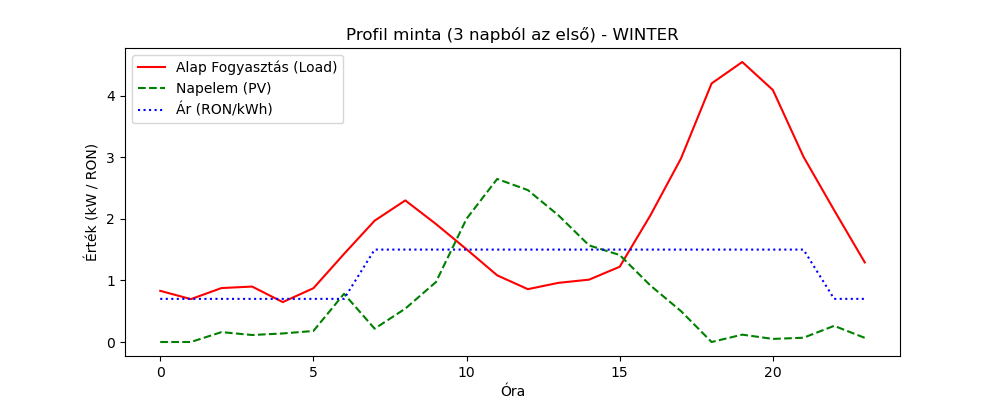
\includegraphics[width=0.85\textwidth]{ekim2339_proj/generated_day_winter.png}
\caption{Téli bemeneti profilok (PV termelés és fogyasztás)}
\label{fig:winter_day}
\end{figure}

\begin{figure}[H]
\centering
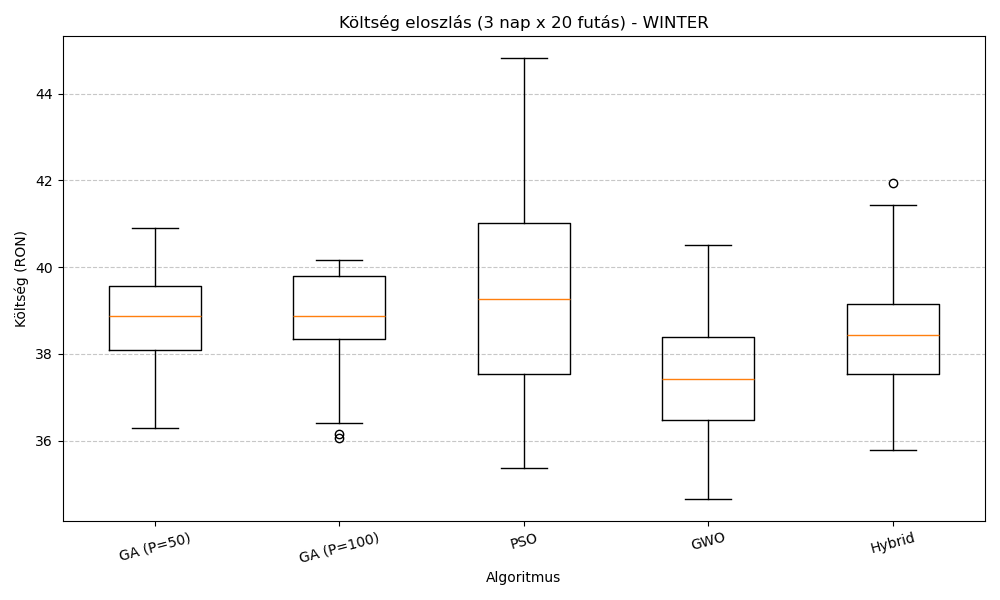
\includegraphics[width=0.85\textwidth]{ekim2339_proj/results_boxplot_winter.png}
\caption{Költség eloszlás a téli szcenárióban (20 futás)}
\label{fig:winter_box}
\end{figure}

\section{A 2x2-es kísérleti mátrix: robusztusság validálása}
\label{sec:matrix_2x2}

Az algoritmusok valódi robusztusságának megismeréséhez az egyszerű szezonális tesztelésből továbblépünk egy szofisztikáltabb megközelítésre: a \textbf{2x2-es kísérleti mátrixra} (PV termelés × Háztartási fogyasztás kombinációja).

\subsection{Motiváció}
A korábbi szintetikus profil-alapú tesztelés biztosított egy "tiszta laborkörnyezetet", ahol az inputok jól szabályozhatók voltak. De az igazi, gyakorlati alkalmazásban az optimalizátornak \textit{egyszerre} kell kezelni:
\begin{itemize}
	\item \textbf{Termelési oldalon}: a valós időjárási adatokból származó, előre nem látható termelésfluktuációkat (felhőzet, napszög),
	\item \textbf{Fogyasztási oldalon}: a valós háztartások sajátos, oft véletlenszerű fogyasztási szokásait (mikróhullámú sütő, mosógép, TV-ezés).
\end{itemize}

Ahhoz, hogy az algoritmusok \textit{generalizálhatóságát} is teszteljük, négy kombinációt érték el:

\begin{table}[H]
\centering
\caption{2x2-es kísérleti mátrix: termelés és fogyasztás kombinációi}
\label{tab:matrix_2x2}
\begin{tabular}{c|cc}
\hline
\textbf{} & \textbf{Szintetikus Load} & \textbf{Valós Load (UCI)} \\
\hline
\textbf{Szintetikus PV} & (1) Lab-ideális & (3) Fogyasztási zaj \\
& Szezonális görbe & Valódi háztartási data \\
\hline
\textbf{Valós PV} & (2) Termelési zaj & (4) Valós Világ \\
& Inverter inverter adatok & Dupla zaj: PV + Load \\
\hline
\end{tabular}
\end{table}

A négy eset, sorrendben:
\begin{enumerate}
	\item \textbf{Szintetikus–Szintetikus (Lab-ideális)}: Az "elméleti maximum" eset. Mind az inverter, mind a fogyasztási terhelés tiszta, szinuszos görbék. Ez az eset azt mutatja meg, hogy az algoritmusok "jó körülmények között" mennyire optimálisak.
	
	\item \textbf{Valós PV–Szintetikus Load}: A termelés valódi inverter-adatok alapján jön (felhős napok, hirtelen fordulatok), de a fogyasztás még tiszta, generált görbe. Ez elkülöníti a \textit{termelési oldal bizonytalanságának} hatását.
	
	\item \textbf{Szintetikus PV–Valós Load}: Az UCI Machine Learning Repository okosóra adatsorából származó, valódi háztartási fogyasztás. A termelés viszont még ideális. Ez a \textit{fogyasztási oldal zaja} (pl. hajszárító, mikróhullámú sütő véletlenszerű bekapcsolása) hatását mutatja meg.
	
	\item \textbf{Valós PV–Valós Load}: A "teljes valóság": mindkét oldal zajos. Ez az a forgatókönyv, ahol az algoritmusnak az összes szabadságfokozat ismeretében kell döntenie.
\end{enumerate}

\subsection{A 2x2-es mátrix tudományos értéke}
Ez a fajta kereszt-validáció az algoritmus-értékelésben már standard a kutatásban (pl. képfeldolgozásban, időjárás-előrejelzésben). A HEMS-kontextusban azonban újszerűnek számít. Az előnye:
\begin{itemize}
	\item \textbf{Szeparáció}: Azonosítható, hogy az algoritmus "zaja" melyik forrásból ered.
	\item \textbf{Generalizálhatóság}: Ha egy algoritmus az (1)-es eseten nyeri, de a (4)-esben lezuhan, az erős indikátor az overfitting-ről.
	\item \textbf{Robusztusság-sorrend}: Az algoritmusok gyakorlati hasznossága nem az elméleti esetből, hanem a (4)-es valós esetet alapján rangsorolható.
\end{itemize}

A mátrix konfigurációja:
\begin{itemize}
	\item 16 kiválasztott nap (4 évszak × 4 nap),
	\item 5 algoritmus (GA-50, GA-100, PSO, GWO, Hybrid),
	\item 2 futás / profil / algoritmus,
	\item 4 kombinációs eset.
\end{itemize}

Összesen: \(16 \times 2 \times 5 \times 4 = 640\) algoritmus-futtatás, amely az algoritmusok teljesítménystabilitásáról ad részletes képet.

\section{Főbb megállapítások}

A kísérletek rávilágítottak a \textbf{szezonális különbségek} fontosságára. Nyáron az optimalizáció kulcsa a többlettermelés menedzselése (az akkumulátor töltése vagy visszatáplálás), míg télen a drága csúcsidőszaki fogyasztás minimalizálása a cél. A vizsgált három szcenárió (tél, nyár, borús) megfelelően lefedi a valós üzemeltetési körülményeket. Az \textbf{algoritmus választást} illetően megállapítható, hogy nincs egyetlen "legjobb" módszer. A GA (P=100) a komplex, változékony esetekben bizonyult robusztusnak, míg a GWO a szigorúbb korlátokkal terhelt téli környezetben működött hatékonyabban. Az \textbf{akkumulátor szerepe} különösen a borús tesztesetben mutatkozott meg, ahol kulcsfontosságúnak bizonyult a termelés ingadozásainak kisimításában. A \textbf{futási teljesítmény} tekintetében az algoritmusok 0.21 és 0.92 másodperc közötti idő alatt találtak megoldást; a PSO volt a leggyorsabb, de ez gyakran a megoldás minőségének rovására ment.

\section{Gazdasági megtérülés}
\begin{table}[H]
\centering
\caption{Beruházási és megtérülési kalkuláció becslés}
\begin{tabular}{lc}
\toprule
\textbf{Tétel} & \textbf{Költség/Érték} \\
\midrule
HEMS hardver & $\approx$ 1200 RON \\
5 kWp napelem rendszer & $\approx$ 15000 RON \\
10 kWh akkumulátor & $\approx$ 18000 RON \\
\midrule
\textbf{Teljes beruházás} & \textbf{$\approx$ 34200 RON} \\
\midrule
Éves megtakarítás (becsült) & $\approx$ 6200 RON \\
\midrule
\rowcolor{yellow!30}
\textbf{Megtérülési idő} & \textbf{$\approx$ 5.5 év} \\
\bottomrule
\end{tabular}
\end{table}
Támogatással (Casa Verde) a megtérülés 3--4 évre csökkenthető.

\section{Környezeti hatás}
A rendszer környezeti hatása jelentős. Az évi 6000 kWh saját napelemes termelés önmagában mintegy 4.8 tonna CO$_2$ kiváltását eredményezi. Ehhez adódik hozzá a terhelés-eltolásból és a hatékonyságnövelésből származó további 2000 kWh megtakarítás, ami újabb 1.6 tonna kibocsátáscsökkenést jelent. \textcolor{red}{\textbf{Összességében így évente nagyságrendileg 6.4 tonna CO$_2$ megtakarítás érhető el.}}

\section{Jövőbeli kutatási irányok és fejlesztési lehetőségek}

A jelenlegi modell továbbfejlesztése több kritikus irányban is lehetséges, amelyek tovább növelhetik a HEMS rendszerek gazdasági és műszaki relevanciáját:

\begin{description}
	\item[Energiaközösségek (REC):] A Peer-to-peer energia-kereskedelem és a közösségi akkumulátor-használat integrálása becsléseink szerint további 10--15\%-os megtakarítást eredményezhet a tagok számára. E modell különösen alkalmazható városi lakóparkok vagy községi szövetkezetek számára.
	
	\item[Többcélú (Multi-objective) optimalizálás:] Olyan Pareto-front alapú megközelítés bevezetése, amely lehetővé teszi a felhasználó számára a költségminimalizálás és a komfortszint közötti adaptív választást, így rugalmasabb vezérlés válik lehetővé.
	
	\item[Gépi tanulás integrációja:] LSTM-alapú (Long Short-Term Memory) időjárás-előrejelzés és a felhasználói szokások folyamatos tanulása a prediktív karbantartás és pontosabb ütemezés érdekében. E megközelítések további 5--10\%-os hatékonyság-javulást eredményezhetnek.
	
	\item[V2G (Vehicle-to-Grid) technológia:] Az elektromos autók mobil akkumulátorként való kezelése, amely a tárolási kapacitást nagyságrendekkel növelheti. Egy 60 kWh-s EV akku 6-szor nagyobb tárolási kapacitást jelent, ami 50--100 RON/hó plusz bevételt generálhat az agregált kereskedelem révén.
\end{description}

E kiterjesztések közül az LSTM-alapú előrejelzés és a V2G már ipari pilóta-projektekben is testesülnek meg (pl. Németország, Hollandia, Dánia), így az elméleti potenciál valósággá válásának az esélye magas.

\section{Implementációs ajánlások és gazdasági szempontok}

A kísérleti eredmények és a piaci adatok alapján a következő javaslatok tehetők a különböző felhasználói csoportok számára:

\begin{description}
	\item[Kis háztartások (< 3 fő):] Számukra egy minimális HEMS konfiguráció javasolt (vezérlő és intelligens konnektorok), amelynek beruházási költsége (800--1200 RON) 1.5--2 év alatt megtérülhet az elérhető 15--20\%-os megtakarítás (évi 500--800 RON) révén. Ezek a háztartások elsősorban a terhelés-eltolásban (pl. mosógép futtatása olcsóbb áras időszakban) találnak lehetőséget.
	
	\item[Közepes háztartások (3--5 fő):] Egy komplettebb rendszer kiépítése ajánlott: HEMS vezérlő + 3--5 kWp-es napelemes rendszer + 5--10 kWh akkumulátor. A 25000--35000 RON-os beruházás (támogatásokkal csökkenthető) 30--50\%-os megtakarítást (évi 3000--5000 RON) eredményez. Megtérülési idő: 3--5 év támogatással, 6--8 év nélküle. Itt az akkumulátor szerepe kritikus a saját termelés hatékony kihasználásában.
	
	\item[Nagy háztartások (> 5 fő):] Teljes rendszer: 5--10 kWp-es napelem + 10--20 kWh sztoráz + felsőbb szintű HEMS. A 40000--60000 RON-os beruházás 50\% feletti megtakarítást (évi 6000--8000 RON) eredményez, így az 3--4 év alatt térül meg támogatásokkal. Ezeken a háztartásokon az egy-két napi akkumulátor-kapacitás lehetővé teszi az intelligens vásárlást az napi áringadozások alapján.
\end{description}

Az implementáció javasolt sorrendje: (1) HEMS vezérlés és adatgyűjtés, (2) Napelemes rendszer telepítés, (3) Akkumulátor-tárolás. Ez a fokozatosság lehetővé teszi a beruházási kockázat csökkentését és a felhasználók fokozatos habitusváltozásának támogatását.

\section{Kódbázis-alapú benchmark-értékelés}
A projekt legfontosabb eredményei a négy szcenáriót vizsgáló, valós és szintetikus adatokat kombináló (2x2) benchmarkból származnak. Ez a futtatás 16 kiválasztott napot, 4 adatváltozatot, 5 algoritmust és 2 ismétlést kombinál, vagyis \textbf{összesen 640 algoritmusfuttatást} értékel.

Az összegzett eredményeket a \ref{tab:realpv_synth_summary}. táblázat foglalja össze, amely jól mutatja az algoritmusok minőség--sebesség kompromisszumát a különböző zajszintek mellett:

\begin{table}[H]
\centering
\caption{A 2x2-es benchmark fő eredményei (640 futtatás aggregációja)}
\label{tab:realpv_synth_summary}
\resizebox{\textwidth}{!}{
\begin{tabular}{llccc}
\toprule
\textbf{Adathalmaz} & \textbf{Algoritmus} & \textbf{Átlagköltség (RON)} & \textbf{Gap \%} & \textbf{Győzelmi arány \%} \\
\midrule
\multirow{5}{*}{\textbf{(1) Lab-ideális} (Synth PV + Synth Load)} 
& \textbf{GA (P=100)} & \textbf{10.50} & \textbf{1.56} & \textbf{62.5} \\
& GA (P=50) & 10.86 & 4.69 & 25.0 \\
& GWO & 11.37 & 10.14 & 12.5 \\
& Hybrid & 13.04 & 27.45 & 0.0 \\
& PSO & 14.02 & 41.00 & 0.0 \\
\midrule
\multirow{5}{*}{\textbf{(2) Termelési zaj} (Real PV + Synth Load)} 
& \textbf{GA (P=100)} & \textbf{13.61} & \textbf{0.96} & \textbf{62.5} \\
& GA (P=50) & 13.90 & 32.08 & 18.8 \\
& GWO & 14.23 & 60.65 & 18.8 \\
& Hybrid & 15.43 & 82.20 & 0.0 \\
& PSO & 16.70 & 159.08 & 0.0 \\
\midrule
\multirow{5}{*}{\textbf{(3) Fogyasztási zaj} (Synth PV + Real Load)} 
& \textbf{GA (P=100)} & \textbf{7.76} & \textbf{2.73} & \textbf{62.5} \\
& GA (P=50) & 7.96 & 3.72 & 31.2 \\
& GWO & 8.77 & 13.15 & 6.2 \\
& Hybrid & 9.79 & 23.30 & 0.0 \\
& PSO & 11.14 & 45.33 & 0.0 \\
\midrule
\multirow{5}{*}{\textbf{(4) Valós világ} (Real PV + Real Load)} 
& \textbf{GA (P=100)} & \textbf{10.80} & \textbf{1.97} & \textbf{50.0} \\
& GA (P=50) & 11.13 & 5.24 & 31.2 \\
& GWO & 11.64 & 17.29 & 18.8 \\
& Hybrid & 13.17 & 44.28 & 0.0 \\
& PSO & 13.92 & 72.32 & 0.0 \\
\bottomrule
\end{tabular}
}
\end{table}

A táblázatból egyértelműen látszik, hogy a \textbf{GA (P=100)} mind a négy adathalmazon robusztus maradt: az átlagos költsége és a gap \% értéke is konzisztensen a legjobb. Ugyanakkor a 4. forgatókönyvben (Valós világ), ahol mind a termelés, mind a fogyasztás magas zajszinttel rendelkezett, a GA(P=100) győzelmi aránya 62.5\%-ról 50.0\%-ra csökkent, ami jelzi a keresési tér drasztikus nehezedését. 
A \textbf{PSO} a laboratóriumi körülmények között még elfogadható lemaradással futott, de a valós, zajos idősorok (különösen a valós PV) bevezetésekor a teljesítménye összeomlott (akár 159\%-os gap). Ez a benchmark validálja, hogy a valós adatok használata kritikus lépés a HEMS algoritmusok tesztelésében.

\section{A bemeneti adatminőség hatása az optimalizációs teljesítményre}
Az egyik legfontosabb mérnöki tanulság, hogy a valós PV-idősor nem csak "szebb bemenet", hanem ténylegesen módosítja az optimalizálási tájképet. A real\_pv futásokban a megoldások költségszórása és az algoritmusok közti gap különbsége nagyobb, vagyis a solvernek nem csupán a terhelés áthelyezését, hanem a napelemtermelés időbeli torzulásait is kezelnie kell.

A synthetic változat ezzel szemben kontrolláltabb környezetet ad: a termelés és fogyasztás generált, ezért a modell belső logikája jobban illeszkedik a keresési stratégiákhoz. Ez nem hibája a modellnek, hanem előnye a vizsgálatnak: így külön látszik, hogy mennyit veszít vagy nyer az algoritmus a bemeneti realizmus növelésével.

\section{Algoritmusok közötti gyakorlati különbségek}
A projekt eredményei nem csak sorrendet, hanem szerepköröket is kijelölnek:
\begin{itemize}
	\item \textbf{GA(P=100)}: a legjobb általános választás, mert stabil és jól kezeli a változó profilokat;
	\item \textbf{GA(P=50)}: jó kompromisszum, ha a futásidő fontosabb, de a stabilitás még kell;
	\item \textbf{GWO}: alacsonyabb paraméterigény mellett is erős alternatíva, különösen zártabb keresési térben;
	\item \textbf{Hybrid}: gyors és kiegyensúlyozott, de a jelen konfigurációban nem hoz minden esetben elég extra javulást;
	\item \textbf{PSO}: a leggyorsabb, de az eredmények alapján a költségoptimalizálásban a leginkább sérülékeny.
\end{itemize}

Ez a szereposztás nagyon fontos, mert a védés során egyértelműen meg lehet mutatni: a projekt nem csupán azt bizonyítja, hogy "melyik a legjobb algoritmus", hanem azt is, hogy különböző üzemeltetési prioritások mellett más-más módszer lehet a legpraktikusabb.

\section{A jelenlegi modell gyakorlati értéke}
A modell még nem végleges ipari rendszer, de tudományos és mérnöki szempontból már most is értékes. Három okból:
\begin{enumerate}
	\item valós árinformációt használ,
	\item elkülöníti a bemeneti realizmus és az algoritmikus teljesítmény hatását,
	\item auditálható, mivel a nyers adatok és az összegző metrikák is mentve vannak.
\end{enumerate}

Ez azt jelenti, hogy a dolgozat következtetései nem "egy futásból származó benyomások", hanem visszakereshető, strukturált benchmark-eredmények.
